\documentclass[11pt, aspectratio = 169]{beamer}

\usetheme[progressbar=frametitle]{metropolis}
\usepackage{appendixnumberbeamer}
\usepackage{booktabs}
\usepackage[scale=2]{ccicons}
\usepackage{pgfplots}
\usepgfplotslibrary{dateplot}
\usepackage{xspace}
\usepackage{hyperref}  
\usepackage{tikz}  
\usetikzlibrary{shapes,decorations,arrows,calc,arrows.meta,fit,positioning}
\tikzset{
    -Latex,auto,node distance =1 cm and 1 cm,semithick,
    state/.style ={ellipse, draw, minimum width = 0.7 cm},
    point/.style = {circle, draw, inner sep=0.04cm,fill,node contents={}},
    bidirected/.style={Latex-Latex,dashed},
    el/.style = {inner sep=2pt, align=left, sloped}
}
\usepackage{verbatim} 
\usepackage{listings}
\newcommand{\themename}{\textbf{\textsc{metropolis}}\xspace}
\definecolor{links}{HTML}{1B1B81}
\hypersetup{colorlinks,linkcolor=blue,urlcolor=blue}

\title{Applied Economics}
\subtitle{Difference-in-Differences Estimator}
\author{Beate Thies}
\date{}
\institute{Winter 2024/25}
% \titlegraphic{\hfill\includegraphics[height=1.5cm]{logo.pdf}}
\setbeamercolor{normal text}{fg=black}
\setbeamercolor{block title}{fg=teal}

\let\svdescription\description
\let\svenddescription\enddescription
\renewenvironment{description}{%
  \svdescription%
  \let\svitem\item%
  \renewcommand\item[1][]{\svitem[\textcolor{\descriptioncolor}{##1}]}%
  }{
  \svenddescription%
  }
\newcommand\descriptioncolor{teal}

\begin{document}

\maketitle

\section{Introduction}

\begin{frame}{Motivation}
    
Multiple regression often does not provide causal estimates because of \color{teal}\textbf{endogeneity}. \color{black}
\begin{itemize}
    \item observational data: subjects are not randomly assigned to treatment ($\neq$ experimental data)
    \item data reflects real life choices -- often correlated with unobservable characteristics
\end{itemize}
%\color{teal}\textbf{Randomized experiments} \color{black} (RCTs) can solve this problem but are often impractical. 

\pause 


There are three widely used \color{teal}\textbf{quasi-experimental methods} \color{black}that intend to \textit{mimic the idea of random treatment assignment:} 
\begin{itemize}
    \item instrumental variables (IV)
    \item differences-in-differences (DiD)
    \item regression discontinuity designs (RDD)
\end{itemize}

\end{frame}

\begin{frame}{Differences-in-Differences}
The DiD approach exploits changes in a policy over time that don't affect everyone to estimate the causal effect of the policy.

\pause 

You need data on 2 groups:
\begin{itemize}
    \item \textbf{control group}: never receives treatment/policy
    \item \textbf{treatment group}: initially untreated and then receives treatment/policy
\end{itemize}

\pause 
You need data for 2 time periods:   \textbf{before and after treatment}. \\
$\rightarrow$ Requires panel data.


Under certain assumptions, the control group can serve as the \textcolor{blue}{counterfactual} for the treatment group. $\rightarrow$ \textbf{Difference in outcomes between groups after vs. before treatment} gives causal effect of interest.
\end{frame}

\section{Example:  Causal effect of Minimum Wage on Employment}

\begin{frame}{Card \& Krueger (1994)}
Why can we not just run a regression of employment rate on minimum wage (MW) at the state level? % (Reverse causality: states introduce/raise MW during good economic conditions)

\pause

\hyperlink{https://davidcard.berkeley.edu/papers/njmin-aer.pdf}{Card and Krueger (1994)} use the DiD approach to estimate the effect of an increase in the MW on the employment rate in the fast-food industry. 

\begin{itemize}
    \item New Jersey (NJ) increased the state MW in 1992 from \$4.25 to \$5.05 per hour \alert{(treatment group)}
    \item Neighboring Pennsylvania (PA) did not change its minimum wage level \\
    \alert{(control group)}
    \item The authors surveyed 410 fast-food establishments in NJ and eastern PA, once  \alert{before} the NJ MW increase (early 1992), and once \alert{after} the NJ MW increase (late 1992)
\end{itemize}
\end{frame}

\begin{frame}{DiD: Idea}
We observe how employment changed in NJ from before to after the increase in the MW. \\
 Does this allow to infer about the causal effect of the MW increase? Why (not)?

 
\pause
To identify the effect of the MW increase on employment, we need a \textcolor{blue}{counterfactual}: \\
How would employment have changed during that time period, \textit{if MW had \textit{not} been increased}?

\pause 


Use time trend in neighboring PA (control group) as counterfactual: in the absence of the policy, we would have expected the same trend in NJ

\begin{itemize}
    \item PA and NJ are very
similar: similar institutions, similar habits, similar consumers, similar incomes, similar weather, etc.
\end{itemize}
%The DID estimator is
\end{frame}



\begin{frame}{DiD Estimator: Basic Form}

    \centering
    \begin{table}
        \caption{Sample Means of Employment (FTE) per Store}
     \\
        \begin{tabular}{lccc}
    \toprule
                           &  NJ & \only<2->{PA} & \\
                           \midrule
         Before Treatment  &  20.4 & \only<2->{23.3} & \\
After Treatment &  21.0 & \only<2->{21.2}  &\\
\midrule
Difference (A-B)& \only<1->{0.6} & \only<2->{-2.1} & \alert{\only<3->{DiD estimate: $0.6 - (-2.1) = 2.7$} }\\
\bottomrule
\end{tabular}
    \end{table}

\end{frame}

\begin{frame}{DiD Estimator: Graphical}
 \only<1>{   \begin{figure}
    \centering
    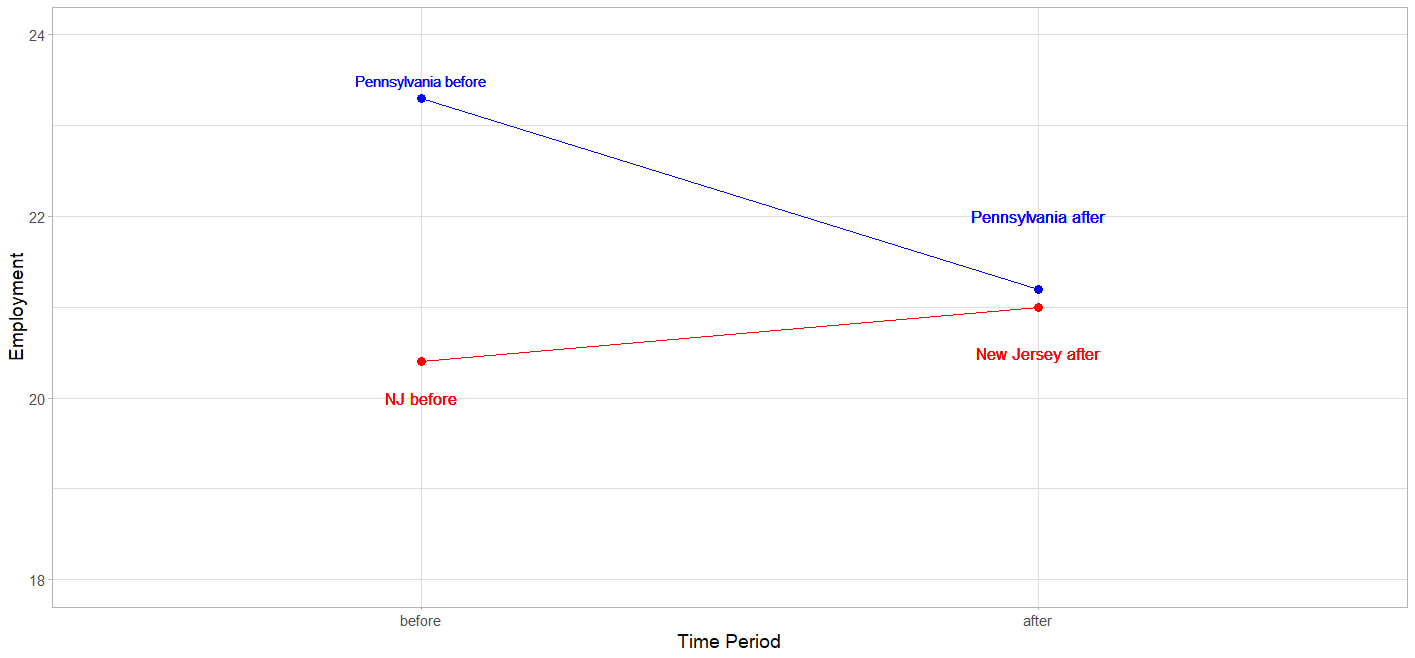
\includegraphics[width=\linewidth]{plot0.png} \end{figure}
 }

     \only<2>{   \begin{figure}
    \centering
    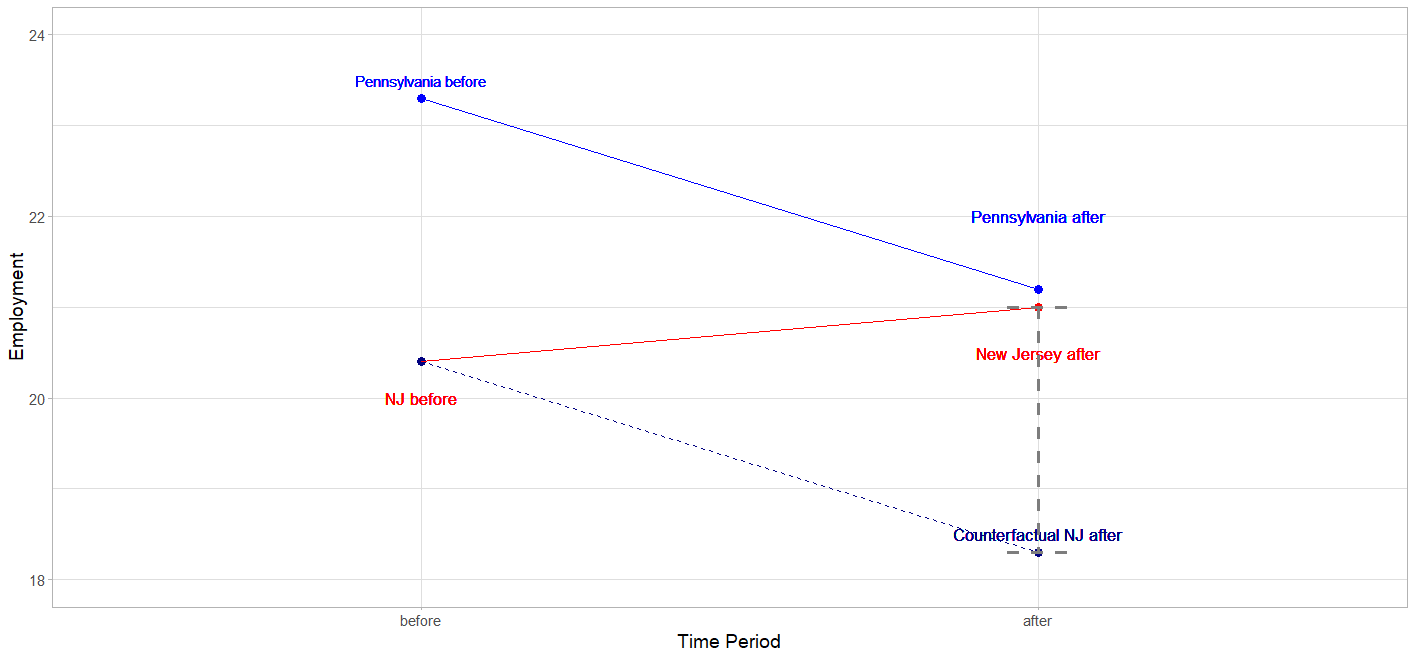
\includegraphics[width=\linewidth]{plot1.png} \end{figure}
}
\end{frame}


\section{Diff-in-Diff Estimator: Basic Form}

\begin{frame}{DiD Estimator: Basic Form}
More generally, the DiD estimator is given as:
\begin{align*}
  \widehat{\beta}^{\text{DiD}} =& \, (\overline{Y}^{\text{treatment,after}} - \overline{Y}^{\text{treatment,before}}) - (\overline{Y}^{\text{control,after}} - \overline{Y}^{\text{control,before}}) \\
  =& \Delta \overline{Y}^{\text{treatment}} - \Delta \overline{Y}^{\text{control}} 
\end{align*}

with
\begin{description}
\item[$\overline{Y}^{\text{treatment,before}}$] sample average in the TG before the treatment \color{gray} $\rightarrow$ $\overline{Employm}^{\text{NJ,before}}$
\item[$\overline{Y}^{\text{treatment,after}}$] \color{black} sample average in the TG after the treatment \color{gray}
$\: \: \: \: \rightarrow$ $\overline{Employm}^{\text{NJ,after}}$
\item[$\overline{Y}^{\text{control,before}}$] \color{black} sample average in the CG before the treatment \color{gray} $\: \: \: \:  \rightarrow$ $\overline{Employm}^{\text{PA,before}}$
\item[$\overline{Y}^{\text{control,after}}$] \color{black} sample average in the CG after the treatment \color{gray} $\: \: \: \: \: \: \: \: \rightarrow$ $ \overline{Employm}^{\text{PA,after}}$
\end{description}
\end{frame}


\begin{frame}{Parallel Trends Assumption}
The crucial assumption to identify the causal effect of interest with the DiD estimator is the \alert{\textbf{Common or Parallel Trends Assumption:}}
\\
\textit{In the absence of treatment, time trends in the treatment group would have been the same as in the control group.}

\pause

Example: absent any minimum wage increase, Pennsylvania's fast-food employment trend would have been what we should have expected to see in New Jersey. $\rightarrow$ trend in PA is a reliable counterfactual for NJ

\pause

It is impossible to validate whether the assumption holds. (By definition, we cannot observe what would have happened in the absence of treatment in the TG) \\
Intuitive check: compare trends $before$ policy change

\end{frame}

\begin{frame}{Parallel Trends Assumption}
    \begin{figure}
        \centering
        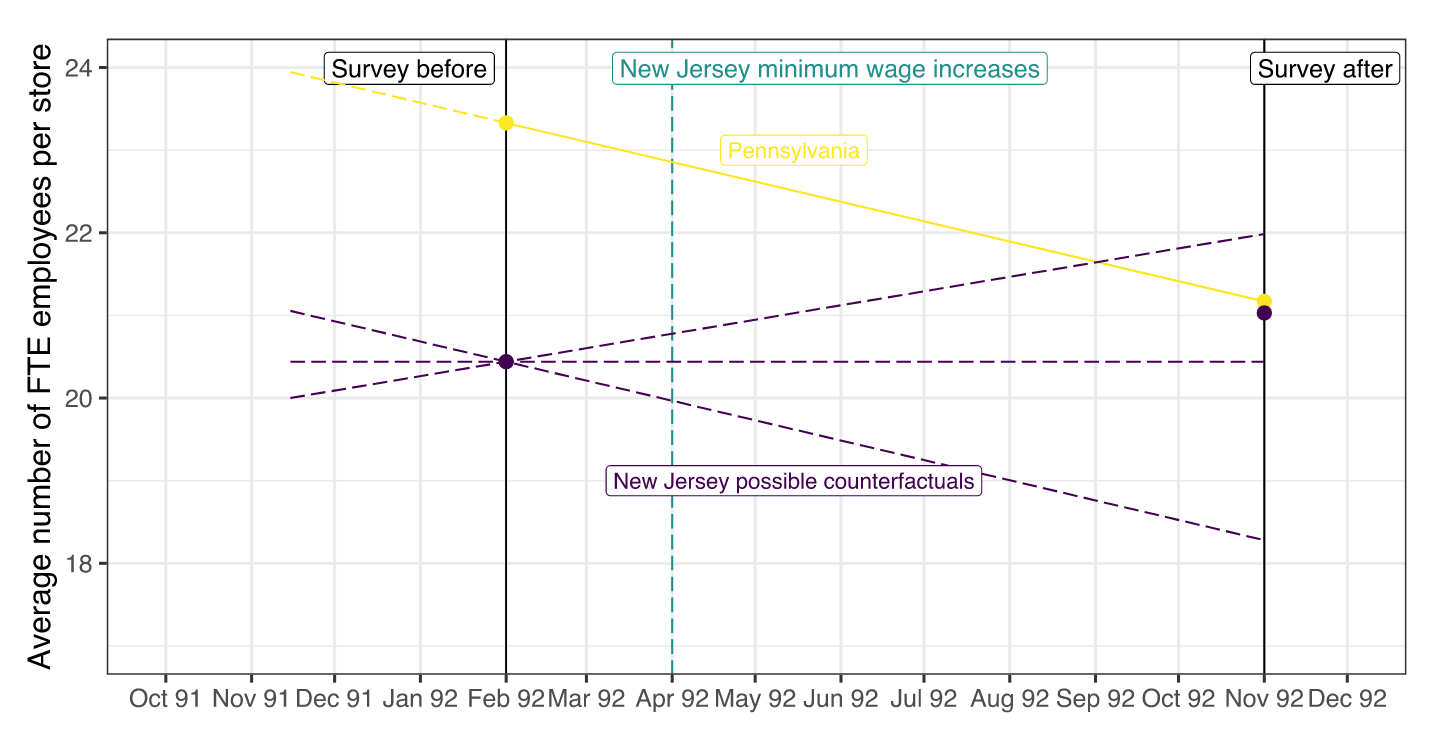
\includegraphics[width=1\linewidth]{didp.png}
        \label{fig:enter-label}
    \end{figure}
\end{frame}
\section{Diff-in-Diff Estimator: \\
Regression Form}

\begin{frame}{Diff-in-Dif Estimator: Regression Form}
In practice, the DiD estimator is usually estimated in a regression format. \\
One can show that the DiD estimate obtained by differencing the sample means is the same as the OLS estimate of $\beta_{TE}$ in
\vspace{-0.02cm}
\begin{align*}
  Y_{it}= & \alpha + \gamma Treat_i + \delta Post_t + \beta_{TE} (Post_t \times Treat_i) + \varepsilon_i 
\end{align*}

\begin{description}
    \item[$Treat_i$] Treatment group dummy, with index $i$ for cross-sectional units (e.g. individual stores)
\item[$Post_t$] Treatment periods dummy, with index $t$ for time periods
\item[$Treat_i \times Post_t$] Interaction term $\rightarrow$ the coefficient $\beta_{TE}$ is the DiD causal effect!
\end{description}
\pause 


Example: \\
$Treat_i$= \begin{cases}
    0 \text{ if $i$ in Pennsylvania}, \\
    1\text{ if $i$ in New Jersey}
\end{cases}
$Post_t$ = \begin{cases}
    0 \text{ if } t < \text{ April 1992,} \\
    1 \text{ if } t \geq \text{ April 1992}
\end{cases}
\end{frame}



\begin{frame}{Understanding the Regression}
\begin{align*}
  Y_{it}=& \alpha + \gamma Treat_i + \delta Post_t + \beta_{TE} (Post_t \times Treat_i) + \varepsilon_i 
\end{align*}

$E(Y_{it}|Treat_i=0,Post_t=0)= \alpha$

$E(Y_{it}|Treat_i=0,Post_t=1)= \alpha + \delta$

$E(Y_{it}|Treat_i=1,Post_t=0)= \alpha + \gamma$

$E(Y_{it}|Treat_i=1,Post_t=1)= \alpha + \gamma  + \delta  + \beta_{TE}$
\small

\hspace{+0.25cm}$\underbrace{[E(Y_{it}|Treat_i=1,Post_t=1)-E(Y_{it}|Treat_i=1,Post_t=0)]}_{\color{teal} \delta + \beta_{TE} = \text{time trend + treatment effect}}-$

\hspace{+0.4cm}$\underbrace{[E(Y_{it}|Treat_i=0,Post_t=1)-E(Y_{it}|Treat_i=0,Post_t=0)]}_{ \color{blue} \delta = \text{time trend}}=\beta_{TE}$

The control group allows to estimate the time trend.
\end{frame}



\begin{frame}{Diff-in-Diff Estimator: Regression Form}

The regression form allows to use more than just two time periods (i.e. multiple periods before and/or after the treatment).

Moreover, one can add additional regressors that measure pre-treatment characteristics to the regression:
\begin{align*}
  Y_{it}=& \alpha + \gamma Treat_i + \delta Post_t + \beta_{TE} (Post_t \times Treat_i) + \pi X_i + \varepsilon_i 
\end{align*}

The additional regressors may lead to a more precise estimate of $\beta_{TE}$.

\end{frame}

\section{Practice}

\begin{frame}{Practice}
Evaluate effect of installation of a garbage incinerator on prices of nearby houses. \\
Did the installation in 1981 cause house prices to drop?
\small

\begin{enumerate}
\item why might a simple comparison of prices of nearby houses before vs. after 1981 not reveal the causal effect of the incinerator?
    \item open dataset \texttt{"diff\_in\_diff.csv"}
    \item generate a POST dummy that takes value 1 if year = 1981 and 0 if year =  1978
    \item generate a TREAT dummy that takes value 1 if house is closer than 5km from the incinerator, using the variable $dist$ (distance to incinerator in meters)
    \item compute sample mean prices for treatment and control houses before and after the treatment 
    \item  compute the diff-in-diff estimator in its basic form. What does it tell you?
    \item formulate the common trends assumption for this analysis
    \item obtain the diff-in-diff estimator in a regression framework
  %  \item add controll variables to the regression for no. of rooms, area, age and distance to central business district ($cbd$). Interpret the coefficient of interest.
\end{enumerate}
    
\end{frame}
\end{document}



